% Created 2023-02-14 mar. 12:39
% Intended LaTeX compiler: pdflatex
\documentclass[letterpaper, 11pt]{article}
                      \usepackage{lmodern} % Ensures we have the right font
\usepackage[T1]{fontenc}
\usepackage[utf8]{inputenc}
\usepackage{graphicx}
\usepackage{amsmath, amsthm, amssymb}
\usepackage[table, xcdraw]{xcolor}
\definecolor{bblue}{HTML}{0645AD}
\usepackage[colorlinks]{hyperref}
\hypersetup{colorlinks, linkcolor=blue, urlcolor=bblue}
\usepackage{titling}
\setlength{\droptitle}{-6em}
\setlength{\parindent}{0pt}
\setlength{\parskip}{1em}
\usepackage[stretch=10]{microtype}
\usepackage{hyphenat}
\usepackage{ragged2e}
\usepackage{subfig} % Subfigures (not needed in Org I think)
\usepackage{hyperref} % Links
\usepackage{listings} % Code highlighting
\usepackage[top=1in, bottom=1.25in, left=1.55in, right=1.55in]{geometry}
\renewcommand{\baselinestretch}{1.15}
\usepackage[explicit]{titlesec}
\pretitle{\begin{center}\fontsize{20pt}{20pt}\selectfont}
\posttitle{\par\end{center}}
\preauthor{\begin{center}\vspace{-6bp}\fontsize{14pt}{14pt}\selectfont}
\postauthor{\par\end{center}\vspace{-25bp}}
\predate{\begin{center}\fontsize{12pt}{12pt}\selectfont}
\postdate{\par\end{center}\vspace{0em}}
\titlespacing\section{0pt}{5pt}{5pt} % left margin, space before section header, space after section header
\titlespacing\subsection{0pt}{5pt}{-2pt} % left margin, space before subsection header, space after subsection header
\titlespacing\subsubsection{0pt}{5pt}{-2pt} % left margin, space before subsection header, space after subsection header
\usepackage{enumitem}
\setlist{itemsep=-2pt} % or \setlist{noitemsep} to leave space around whole list
\author{Thomas Lebrat}
\date{\textit{<2023-01-31 mar.>}}
\title{Devoir maison}
\begin{document}

\tableofcontents



\section{Exercice - Formation d'un nuage}
\label{sec:org0a706fb}

On souhaite expliquer la formation d'un nuage d'une manière simplifiée. Nous faisons l'hypothèse que son apparition est d'abord conditionnée par un \textbf{\textbf{déplacement adiabatique de masse d’air}}. \footnote{On ommet volontairement certains phénomènes subtiles dans cette première approche (nucléation, ...)}. Cet exercice vous propose tout d'abord d'essayer de résoudre ce problème à partir des équations de base régissant le comportement d'un gaz parfait, puis de réaliser une recherche documentaire sur internet pour essayer d'illustrer ce phénomène d'une manière vulgarisée.

Un point de l'atmosphère est repéré par ses coordonnées cartésiennes (Oxyz), tel que l'axe (Oz) coïncide avec la verticale ascendante avec \(z=0\) pris au niveau de la mer. Par comodité, nous garderons les notations et valeurs numériques des constantes physiques utilisées pour le \texttt{TP 1}. Vous êtes invités à réutiliser des résultats, démonstrations, ou valeurs numériques trouvés en séance.

\subsection{En l'abscence de mouvement (équilibre)}
\label{sec:orgb66527b}

Des relevés expérimentaux montrent qu'en l'absence de mouvement de l'air, la température est fonction de l'altitude \(z\) suivant une loi affine : 

$$ T(z) = T_{0} - \lambda z $$

\textbf{Q1}. (1 pt) Sur quelle intervalle de z cette approximation est-elle valable ?

\newpage

Avec les hypothèse thermodynamiques faites en début de TP, on peut montrer que \(P\) et \(T\) sont liées par une relation de la forme : 

$$ T =T_0 \left( \frac{P}{P_0}  \right)^{q} $$

\textbf{Q2}. (2 pt) En combinant 3 hypothèses portant sur le fluide (statique, GP, hypothèse sur T) , essayez de construire une équations différentielle portant sur la pression \(P\). Tentez ensuite de retrouver cette relation par intégration avec une méthode de séparation des variables.

\textbf{Q3}. (1 pt) Déterminer l’exposant \(q\) qui s'exprime uniquement en fonction de \(M\), \(g_0\), \(\lambda\) et \(R\). Faites l'application numérique pour une valeur convenablement choisie de \(\lambda\).


\subsection{Apparition d'un mouvement (instabilté)}
\label{sec:org300707c}

L'état d'équilibre précédent est réalisé lorsque les isothermes (niveaux où \(T=Cte\)) et les isobares (\(P=Cte\)) coïncident avec les équipotentielles du champ de pesanteur (\(z = cte\))\footnote{les spécialistes parlent de configurations barotropes et baroclines}. En présence d’hétérogénéités de température au niveau du sol, l'air s'échauffe différemment et peut se mettre en mouvement.

\bigskip

\begin{figure}[htbp]
\centering
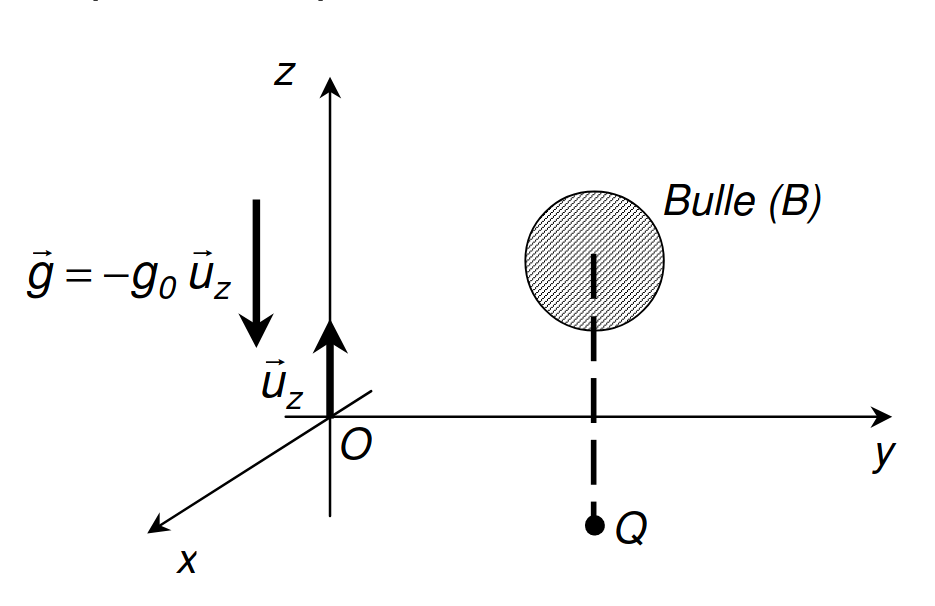
\includegraphics[width=.9\linewidth]{./Ex2a.png}
\end{figure}

On se place à l'altitude \(z\) à la verticale du point \(Q\) et on suppose que l'air est localement plus chaud que l'air avoisinant. Tout se passe comme si une poche de gaz était limitée par une enveloppe souple et non tendue. On convient des hypothèses et notations suivantes : 

\begin{itemize}
\item La bulle de gaz évolue sans échanger de matière ni de chaleur avec l'extérieur.

\item La \textbf{pression de la bulle} reste égale à celle de l'air environnant à la même altitude.

\item La \textbf{température de l'air} environnant varie toujours linéairement avec la température.

\item On note \(P_B\), \(T_B\) et \(\rho_B\) la pression, la température et la masse volumique du gaz emprisonné dans la bulle. On note \(T_A\) et \(\rho_A\) la température et la masse volumique de l'air environnant à la même altitude.
\end{itemize}

\textbf{Q4}. (2 pt) Montrer en raisonnant au départ sur les forces qu'une différence de température entre \(B\) et \(A\) ( \(T_B > T_A\) ) implique une élévation de le bulle \ldots{}

Le gaz emprisonné dans la bulle subit une transformation dite \textbf{adiabatique} et  \textbf{réversible} (ce n'est pas rigouresuememnt vrai mais on fait cette hypothèse simplificatrice pour mettre le problème en équation). Appellons \(T_1\) la température du gaz dans la bulle à l'altitude de sa formation \(z_1\) et \(P_1\) la pression correspondante.

\textbf{Q5}. (2 pt) En retrouvant une des 3 formes de l'expression de la \textbf{loi de Laplace} pour les gaz parfaits, exprimer \(T_B\) en fonction de \(T_1\), \(P_1\) et \(P_B\). \footnote{En cas de difficulté, vous pouvez bien sûr consulter des ressources pour résoudre cette question théorique (notion au programme de thermo de L1 ; pensez à citer vos sources !)}

\textbf{Q6}. (2 pt) On veut démontrer qu'il existe une altitude plafond \({z^{\star}\) pour l'ascension de la bulle. On note \(T^{\star}\) et \(P^{\star}\) la température et la pression de la bulle lorsqu'elle arrive à cette altitude. Evaluer numériquement \(T^{\star}\) et \(P^{\star}\) pour \(T_1 = 280 K\) et \(z_1 = 2 km\). En déduire la valeur de l'altitude plafond \(z^{\star}\) à laquelle se stabilise la bulle.

Pour cette question, on vous demande de rédiger soigneusement une explication du phénomène de stabilisation de la bulle d'air.

\newpage


\subsection{Explication qualitative de la formation d'un nuage.}
\label{sec:org636316b}

\textbf{Q7} (5 pt) Nous faisions l'hypothèse d'un air sec dans la partie précédente. Maintenant nous envisageons une parcelle d'air \emph{humide} (air sec + vapeur d'eau). 

\begin{itemize}
\item Proposer une explication qualitative de la possibilité de formation d'un nuage au cours de l'ascension d'une bulle.

\item Réaliser un schéma légendé, si possible au format A3 \footnote{2 feuilles A4 accolées feront l'affaire}, présentant une illustration vulgarisée de la formation d'un nuage telle qu'on peut la comprendre \textbf{d'après le mécanisme illustré par cet exercice}.

\item Au besoin, ajouter quelques détails supplémentaire (avec une autre couleur) signalant d'autres phénomènes pouvant rentrer en jeu dans le mécanisme de formation d'un nuage.
\end{itemize}
\end{document}
